%****************************************************************************%
%* DIET User's Manual workflow chapter file                                 *%
%*                                                                          *%
%*  Author(s):                                                              *%
%*    - Abdelkader Amar (Abdelkader.Amar@ens-lyon.fr)                       *%
%*    - Raphael Bolze (Raphael.Bolze@ens-lyon.fr)                           *%
%*                                                                          *%
%* $LICENSE$                                                                *%
%****************************************************************************%

\chapter{Workflow management in \textsc{Diet}}

\section{Quick start}


\paragraph{Requirements and compilation}

The workflow supports in \textsc{DIET} needs the following:

\begin{itemize}
\item The Xerces library: the XML handling code is written with
  Xerces-C++ using the provided DOM API.
\item Enable the workflow support when compiling DIET.
\end{itemize}

To build DIET with workflow support using \textit{cmake}, two
configuration parameters need to be set:

\begin{itemize}
\item DIET\_USE\_WORKFLOW as follow: -DDIET\_USE\_WORKFLOW:BOOL=ON
\item XERCES\_HOME: defines the path to Xerces installation directory.
  (for example -DXERCES\_HOME:PATH=/usr/local/xerces)
\end{itemize}

This is an example of generating command line:

\verb|cmake .. -DMAINTAINER_MODE:BOOL=ON -DOMNIORB4_DIR=/usr/local/omniORB \|

\verb|      -DDIET_USE_WORKFLOW:BOOL=ON \|

\verb|      -DXERCES_HOME=/usr/local/xerces|


\paragraph{}
Workflow support was tested in the following configurations:

\begin{itemize}
\item gcc version 4.0.2 and higher.
\item \textit{Xerces} 2.7.
\end{itemize}

%\subsubsection{Previous version \todo{TO REMOVE}}
%
%\paragraph{Compilation using the autotools}
%
%The workflow supports in \textsc{DIET} needs the following:
%
%\begin{itemize}
%\item The QT4 library: the XML handling code is written with
%  QT4 using the provided DOM API.
%\item enable the workflow support by passing the
%  \verb|--enable-workflow| to the configure script.
%\end{itemize}
%
%To specify the QT4 installation directory, you can use the options
%\verb|--with-qt-inc| and \verb|--with-qt-lib| which indicate
%respectively where find headers and libraries. When QT4 is installed
%by binaries (RPM or APT package), the include directory is
%\verb|/usr/include/qt4|, when the library directory is
%\verb|/usr/lib|.
%
%Workflow support was tested in the following configurations:
%
%\begin{itemize}
%\item with FAST
%\item with or without cori support
%\end{itemize}
%
%\paragraph{Compilation using CMake}
%
%To build DIET with workflow support using \textit{cmake}, three
%configuration parameters need to be set:
%
%\begin{itemize}
%\item DIET\_USE\_WORKFLOW as follow: -DDIET\_USE\_WORKFLOW:BOOL=ON
%\item QT\_INC: defines the path to QT4 header, by default set to
%  /usr/include. (for example -DQT\_INC:PATH=/usr/include/qt4)
%\item QT\_LIB: defines the path to QT4 library, by default set to
%  /usr/lib. (for example -DQT\_LIB:PATH=/usr/local/lib)
%\end{itemize}
%
%This is an example of generating command line:
%
%\verb|cmake .. -DOMNIORB4_DIR=/usr/local/omniORB -DDIET_USE_WORKFLOW:BOOL=ON \|\verb 
%\verb|-DQT_LIB:PATH=/usr/lib -DQT_INC:PATH=/usr/include/qt4/| %|

\paragraph{Executing the examples}
%\label{sec:wf_examples}

The directory \texttt{examples/workflow} includes some examples of
workflows.  You can find a simple workflow (see
figure~\ref{fig:example1}) in the file \texttt{xml/scalar.xml} and you
can test it with the following command:

\verb|./scalar_client local_client.cfg scalar.xml |

You need to have a running DIET platform with the needed services. You
can launch separate SeDs (\textit{succ}, \textit{double}, \textit{sum}
and \textit{square}) or a single SeD that includes all the needed
services.

\begin{figure}[htbp]
  \centering
  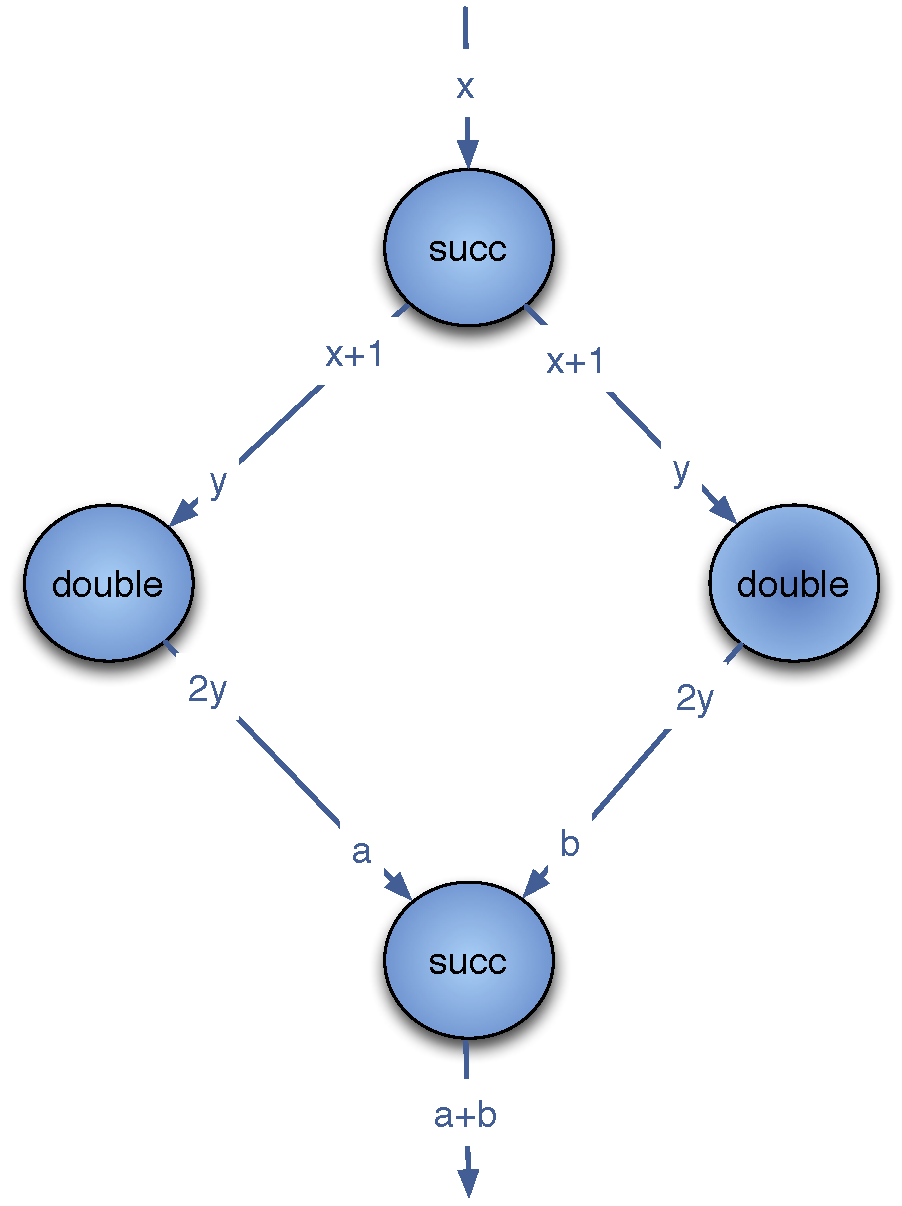
\includegraphics[keepaspectratio,width=0.4\linewidth]{fig/wf_example1}
  \caption{Workflow example}
  \label{fig:example1}
\end{figure}

\section{Software architecture}

The workflow support in \textsc{DIET} provides two architectures and
can be used in three modes.
\begin{itemize}
\item The first one provides a workflow manager in the client side.
\item The second one use a special agent called the \textit{MA\_DAG}
  which is responsible to communicate with the \textit{Master Agent} of
  the platform and provide an ordering and mapping for workflow
  execution.
\item The third mode is similar to the second one, but in this mode
  the \textit{MA\_DAG} provides only an ordering for the workflow
  execution.
\end{itemize}

\subsection{Architecture 1 : Workflow manager inside the client}
\label{sec:archi1}

In this scheme (figure~\ref{fig:archi1}), the handling of workflow is
done by the client, and the execution don't require an MA\_DAG. The
execution steps are~:

\begin{enumerate}
\item The client read and process the workflow description; a dag
  structure is created.
\item The client send a set of the problem descriptions to the
  Master Agent to check if all services are available.
\item If all services are available, the client start the workflow
  execution. By default a random scheduler is used to execute the Dag,
  so only data dependencies are used to define the execution order.
  Between the ready nodes, the invocation order is random. In this
  mode, since all scheduling operation are done in the client side, we
  can use a customized scheduler. The client programmer can write a
  personal scheduler which must be a \textit{AbstractScheduler}
  subclass and implements the \textit{execute} method (for more
  details see the section~\ref{sec:wf_sched}).
\item If the execution was successful, the client can retrieve the
  results.
\end{enumerate}

To use this execution mode, nothing needs to be configured except that
the client configuration file must not include an MADAGNAME parameter.

\begin{figure}[htbp]
  \centering
  \includegraphics[keepaspectratio,width=0.7\linewidth]{fig/wf_archi1}
  \caption{Architecture 1 : workflow manager inside the client}
  \label{fig:archi1}
\end{figure}



\subsection{Architecture 2: Workflow manager = MA DAG}
\label{sec:archi2}

The second architecture (figure~\ref{fig:archi2}) of workflow
management in DIET use an additional entity called the \textit{MA DAG}
to handle the workflow. This agent can work in two modes, in the first
it defines a complete scheduling of the workflow (ordering and
mapping), while in the second it defines only an ordering for the
workflow execution, the mapping is done in the next step by the client
which pass by the Master Agent to find the server where execute the
workflow services.


To use the \textit{MA DAG}, the client configuration file must include
the parameter \textit{MADAGNAME} with the appropriate name.

\paragraph{First mode : the MA\_DAG provides a complete scheduling}

\begin{enumerate}
\item The client sends the workflow description (in a textual format)
  to the MA\_DAG.
\item The MA\_dAG request the platform Master Agent to check if all
  services are available.
\item If the workflow can be executed, the MA\_DAG defines a mapping and
  ordering and send it back to the client. Currently, the ordering is
  random like in the first architecture, while the mapping use a round
  robin policy.
\item The client start the workflow execution and retrieve the results
  if the execution was successful.
\end{enumerate}

When the \textit{MADAGNAME} is set in the configuration file, this is
the default mode. The client can ensure this mode by the method
\texttt{set\_ma\_dag\_sched}. 

\paragraph{Second mode : the MaDag provides only an ordering}

This mode is similar to the previous one, except that the MaDag
provides only an execution order (or a priority tag for each node),
the mapping is done when the client tries to execute each service, so
the server is the one chosen by the Master Agent when requested by the
client.

To use this mode, the client needs to use to the method
\texttt{set\_ma\dag\_sched(0)}. 

\begin{figure}[htbp]
  \centering
  \includegraphics[keepaspectratio,width=0.7\linewidth]{fig/wf_archi2}
  \caption{Architecture 2 : The MA\_DAG as an external workflow manager}
  \label{fig:archi2}
\end{figure}




\section{Client API}


\subsection{Structure of client program}
\label{sec:client_prg}

The structure of a client program is very close to the structure of
usual DIET client. The general structure is as follow:

\begin{verbatim}
diet_initialize

create the workflow profile

call the method diet_wf_call

if success retrieve the results

free the workflow profile

diet_finalize
\end{verbatim}

The table~\ref{tab::wf_api} shows a description of the different
methods provided by diet workflow API. 

\begin{table}[htbp]
  \centering
  \begin{tabular}[htbp]{|p{8cm}|p{7.5cm}|}\hline
    Workflow function & Description \\\hline
    %
    \texttt{diet\_wf\_desc\_t*  \newline
      diet\_wf\_profile\_alloc(const char* wf\_file\_name);} 
    &
    allocate a workflow profile to be used for a workflow submission.\newline
    \textit{wf\_file\_name} : the file name containing the workflow XML description.
    \\\hline
    % 
    \texttt{void  \newline
      diet\_wf\_profile\_free(diet\_wf\_desc\_t * profile);} 
    &
    free the workflow profile.
    \\\hline
    %
    \texttt{diet\_error\_t \newline
      diet\_wf\_call(diet\_wf\_desc\_t* wf\_profile);} 
    &
    execute the workflow associated to profile \textit{wf\_profile}.
    \\\hline
    %
    \texttt{int   \newline
      diet\_wf\_scalar\_get(const char * id, void** value);} 
    &
    Retrieve a workflow scalar result. \newline
    \textit{id} : the output port identifier.
    \\\hline
    % 
    \texttt{int   \newline
      diet\_wf\_string\_get(const char * id, char** value);} 
    &
    Retrieve a workflow string result. \newline
    \textit{id} : the output port identifier.
    \\\hline
    %
    \texttt{int    \newline
      diet\_wf\_file\_get(const char * id, size\_t* size, char** path);
    }
    &
    Retrieve a workflow file result. \newline
    \textit{id} : the output port identifier.
    \\\hline
    % 
    \texttt{int \newline
      diet\_wf\_matrix\_get(id, (void**)value, nb\_rows, nb\_cols, order)
    }
    &
    Retrieve a workflow matrix result. \newline
    \textit{id} : the output port identifier.
    \\\hline
    % 
    \texttt{void \newline
      set\_madag\_sched(int b);}&
    Define if the client use the Ma\_Dag ordering and mapping when
    executing the workflow ($b\neq1$) or just the ordering ($b=0$)
    \\\hline
    %
    \texttt{void  \newline
      set\_sched (struct AbstractWfSched * sched);}&
    Define a customized scheduler defined by the user. The Scheduler
    must be an AbstractScheduler subclass and implements the
    \textit{execute} method.
    \\\hline
    %
    \texttt{void \newline
      enable\_reordering(const char * name, int b);
    }
    & 
    enable/disable the reordering \newline
    reordering enabled (b = true) \newline
    reordering disabled (b = false)
    \\\hline
    %
    \texttt{void \newline
      void get\_all\_results();}
    &
    print all the results of the current executed workflow.
    \\\hline
    %
  \end{tabular}
  \caption{Diet workflow API}
  \label{tab::wf_api}
\end{table}


\subsection{Workflow description}
\label{sec:workflow_desc}

The workflow is described using an XML representation which is close
to diet profile representation. In addition to profile description
(problem path and arguments), this description represents also the
data dependencies between ports (source/sink), the node identifier
(unique) and the precedences between nodes. This last information can
be removed since it can be retrieved from the dependencies between
ports, however it can be useful to define a temporal dependency
without port linking.

The general structure of this description is:

\begin{verbatim}
<dag>
  <node id="..." path="...">
    <arg name="..." type="........" value=".."/>
    <in name="..." type="........" source="......."/>
    <out name="...." type="........" sink="......"/>
    <out name="...." type="........" sink="......"/>
  </node>
  ....
\end{verbatim}

The name argument represents the identifier of the port. To use it to
define a \textit{source} or a \textit{sink} value, it must be prefixed
with the node id. For example if the source of the input port
\textit{in3} is the port \textit{out2} of the node \textit{n1}, than
the element must be described as follow:

\begin{verbatim}
    <in name="in3" type="DIET_INT" source="n1#out2"/>
\end{verbatim}

The example shown in figure~\ref{fig:example1} can be represented by
this XML description:

\begin{verbatim}
<dag>
  <node id="n1" path="succ">
    <arg name="in1" type="DIET_INT" value="56"/>
    <out name="out1" type="DIET_INT" sink="n2#in2"/>
    <out name="out2" type="DIET_INT" sink="n3#in3"/>
  </node>
  <node id="n2" path="double">
    <prec id="n1"/>
    <in name="in2" type="DIET_INT" source="n1#out1"/>
    <out name="out3" type="DIET_INT" sink="n4#in4"/>
  </node>
  <node id="n3" path="double">
    <prec id="n1"/>
    <in name="in3" type="DIET_INT" source="n1#out2"/>
    <out name="out4" type="DIET_INT" sink="n4#in5"/>
  </node>
  <node id="n4" path="sum">
    <prec id="n2"/>
    <prec id="n3"/>
    <in name="in4" type="DIET_INT" source="n2#out3"/>
    <in name="in5" type="DIET_INT" source="n3#out4"/>
    <out name="out4" type="DIET_INT"/>
  </node>
</dag>
\end{verbatim}

\subsection{Examples}
\label{sec:examples}


\subsubsection{Example 1 : the simplest example}
\label{sec:ex1}

This examples represents the basic client code to execute a workflow.
The line 26 indicates that the workflow output is a double value named
\verb|n4#out4|. The example shown in figure~\ref{fig:example1} can be
fully (execution and result retrieving) executed with this client.

\begin{lstlisting}{1}
#include <string.h>
#include <unistd.h>
#include <stdlib.h>
#include <stdio.h>
#include <sys/stat.h>

#include "DIET_client.h"

int main(int argc, char* argv[])
{
  diet_wf_desc_t * profile;
  char * fileName;
  long * l; 
  if (argc != 3) {
    fprintf(stderr, "Usage: %s <file.cfg> <wf_file> \n", argv[0]);
    return 1;
  }
  
  if (diet_initialize(argv[1], argc, argv)) {
    fprintf(stderr, "DIET initialization failed !\n");
    return 1;
  } 
  fileName = argv[2];
  profile = diet_wf_profile_alloc(fileName);
  if (!diet_wf_call(profile)) {
    printf("get result = %d ", diet_wf_scalar_get("n4#out4", &l));
    printf("%ld\n", (long)(*l)); 
  }
  diet_wf_free(profile);
  return 0;
}
\end{lstlisting}

\paragraph{Example 2 :  Use the MA DAG modes}

This example is similar to the previous one but the user can specify
which mode he wants to use by command line options \verb|-madag_sched|
(the default) or \verb|-notmadag_sched|.

\begin{lstlisting}{2}
#include <string.h>
#include <unistd.h>
#include <stdlib.h>
#include <stdio.h>
#include <sys/stat.h>
#include "DIET_client.h"

void usage(char * s) {
  fprintf(stderr, "Usage: %s <file.cfg> <wf_file> [option]\n", s);
  fprintf(stderr, "option = -madag_sched | -notmadag_sched\n");
  exit(1);
}
int checkUsage(int argc, char ** argv) {
  if ((argc != 3) && (argc != 4)) {
    usage(argv[0]);
  }
  if (argc == 4) {
    if (strcmp(argv[3], "-madag_sched") && 
	strcmp(argv[3], "-notmadag_sched")) {
      usage(argv[0]);
    }
  }
  return 0;
}

int main(int argc, char* argv[])
{
  diet_wf_desc_t * profile;
  char * fileName;
  long * l; 
  checkUsage(argc, argv);
  if (diet_initialize(argv[1], argc, argv)) {
    fprintf(stderr, "DIET initialization failed !\n");
    return 1;
  } 
  fileName = argv[2];
  if (argc == 4)
    set_madag_sched(!strcmp(argv[3], "-madag_sched"));
  profile = diet_wf_profile_alloc(fileName);
  if (!diet_wf_call(profile)) {
    printf("get result = %d ", diet_wf_scalar_get("n4#out4", &l));
    printf("%ld\n", (long)(*l)); 
  }
  diet_wf_free(profile);
  return 0;
}
\end{lstlisting}


\section{Scheduling}


\subsection{Available schedulers}

The available schedulers are:

\begin{itemize}
\item In the client: a round robbin and HEFT scheduler.
\item In the MA\_DAG: a round robbin, HEFT, and FOFT (Fairness On
  Finish Time: in multiworkflow support -experimental-).
\end{itemize}

\subsection{Writing a new scheduler}

The workflow scheduler of the client is different little bit from the
MA\_DAG one. To write a new scheduler you need diet sources. The
following two section show how to develop your own scheduler and how
to plug it in your client or in the MA\_DAG.

\paragraph{Client scheduler}

To write a new workflow scheduler for your diet client you need to
create a derived class of the base abstract class
\textit{AbstractWfSched}. The main function of the scheduler (the SeDs
mapping) must be placed in the pure virtual function \textit{execute}.
These are the steps to follow:

\begin{enumerate}
\item Write a subclass of \textit{AbsWfSched} abstract class. The
  virtual method \textit{execute} needs to be implemented.
\item Create a c++ file where you can put the following code:
\begin{verbatim}
extern "C" {
  void set_my_personal_sched() {
    Personal_WfSched * mySched = new Personal_WfSched();
    set_sched(mySched);
  }
}
\end{verbatim}
\item In your client source code, call the method
  \textit{set\_my\_personal\_sched} before executing the
  \textit{diet\_wf\_call}.
\item Link the previous c++ object code to you DIET client.
\end{enumerate}

